\section{Properties of the Wigner distribution}
\label{app:wigner}

Here we present important properties of the Wigner distribution that are used throughout the paper.

\begin{proposition}\label{thm:wstate}
    The Wigner distribution of a state $\rho$ is
    \begin{enumerate}
        \item\label{en:w1} Real valued: $\W{\rho} \in \mathbb{R}^{d^2}$;
        \item\label{en:w2} Normalised: $\sum_{\bmz \in \pd} \W[\bmz]{\rho}=1$;
        \item\label{en:w3} Bounded: $\abs{\W[\bmx]{\rho}} \leq \frac{1}{d}$.
        \item\label{en:w4} Additive under mixing:
        
        $\W[\bmx]{\sum_i p_i \rho_i} = \sum\limits_i p_i \W[\bmx]{\rho_i}$;
        \item\label{en:w5} Multiplicative under tensor products: 
        
        $\W[\bmx_A \oplus \bmx_B]{\rho_A \otimes \rho_B} = \W[\bmx_A]{\rho_A}\W[\bmx_B]{\rho_B}$.
	\end{enumerate}
\end{proposition}
A distribution satisfying the first three properties does not necessarily correspond to a positive semi-definite state.

\begin{proposition}
    \label{thm:wchannel}
    The Wigner distribution of a $\cptp$ operation $\E: \cal{B}(\hd[d_A]) \mapsto \cal{B}(\hd[d_B])$ is:
    \begin{enumerate}
        \item\label{en:wo1} Real-valued: $\W[\bmy|\bmx]{\E} \in \mathbb{R}$;
        \item\label{en:wo2} Normalised: $\sum_{\bmz \in \pd[d_B]} \W[\bmz|\bmx]{\E} = 1$ for any $\bmx \in \pd[d_A]$;
        \item\label{en:wo3} Bounded: $\abs{\W[\bmy|\bmx]{\E}} \leq \frac{d_A}{d_B}$;
	    \item\label{en:wo4} \nick{Transitive}: $\W[\bmy]{\E(\rho)} = \sum_{\bmz \in \pd[d_A]} \W[\bmy|\bmz]{\E} \W[\bmz]{\rho}$ for any $\bmy \in \pd[d_B]$.
    \end{enumerate}
\end{proposition}
If $d_A = d_B$, and in particular if operation $\E$ maps a Hilbert space onto itself, then the stochasticity condition $\abs{\W[\bmy|\bmx]{\E}} \leq 1$ is satisfied.

%%%

\section{Properties of majorization}
\label{app:major}

\subsection{Equivalent conditions for majorization}

Any $\bmd$-majorization problem can be rephrased as a majorization problem in a higher dimensional space due to the embedding map.
\begin{definition}
    The embedding map $\Gamma_{\bmd}:\mathbb{R}^n \mapsto \mathbb{R}^D, D = \sum\limits_{i=1}^n d_i$ is the function
    \begin{equation}
        \Gamma_{\bmd}(\bmz) = \bigoplus_{i=1}^n z_i\  \frac{1}{d_i}\bm{1},
    \end{equation}
    where $\bm{1}/d_i$ is the $d_i$-dimensional uniform distribution.
    The left inverse $\Gamma_{\bmd}^{-1}: \mathbb{R}^D \mapsto \mathbb{R}^n$ is defined to sum up the elements in each block of $\Gamma_{\bmd}(\bmz)$, so that
    \begin{equation}
        \Gamma_{\bmd}^{-1}(\oplus_{i=1}^n z_i \bm{1}/d_i) = \bmz.
    \end{equation}
    This is not a right inverse, because $\Gamma_{\bmd}$ is not surjective.
\end{definition}
The direct sum simply amounts to listing the uniform distributions one after the other.
The embedding map maps the Gibbs distribution to the uniform distribution, $\Gamma_{\bmd}(\bmd) = \bm{1}/D$.
Then, a non-increasing ordering $\Gamma_{\bmd}(\bmz)^\downarrow$ in the new space, corresponds to the so-called ``$\beta$-ordering'' of the original vector denoted by the permutation $\pi$ mapping $(z_i/d_i) \mapsto (z_i/d_i)^\downarrow$ for all $i=1,\dots,n$.
Intuitively, $\beta$-ordering tends to simply non-increasing ordering as $\beta$ tends to 0.
This ordering naturally leads to a generalised notion of the Lorenz curve. 

\begin{theorem}
Given $\bmx, \bmy, \bmd \in \mathbb{R}^n$, such that the components of $\bmd$ are positive, the following statements are equivalent:
 \begin{enumerate}%[\rm{(TM1)}]
	\item $\bmx \prec_{\bmd} \bmy$;
	\item $\Gamma_{\bmd}({\bmx}) \prec \Gamma_{\bmd}({\bmy})$;
	\item\label{en:tm3} $\sum\limits_{i=1}^n \abs{x_i - t d_i} \leq \sum\limits_{i=1}^n \abs{y_i - t d_i}$ for all $t \in \mathbb{R}$;
	\item $\sum\limits_{i=1}^n (x_i - t d_i)^+ \leq \sum\limits_{i=1}^n (y_i - t d_i)^+$ for all $t \in \mathbb{R}$ and $\sum\limits_{i=1}^n x_i = \sum\limits_{i=1}^n y_i$;
	\item $\forall k, L_{\bmx|\bmd}(k) \leq L_{\bmy|\bmd}(k)$ and $L_{\bmx|\bmd}(k=n) = L_{\bmy|\bmd}(k=n)$.
 \end{enumerate}
\end{theorem}
\begin{proof}
    \begin{enumerate}
        \item[1$\leftrightarrow2$]
        Suppose now there exists a stochastic $S$ such that $\bmx = S\bmy$ with $\bmd = S\bmd$ and let $B = \Gamma_{\bmd} \circ S \circ \Gamma_{\bmd}^{-1}$.
        $B$ is a $D$-dimensional bistochastic matrix, since composition of stochastic matrices is stochastic and $(\Gamma_{\bmd} \circ S \circ \Gamma_{\bmd}^{-1}) (\frac{1}{D}\bm{1}) = (\Gamma_{\bmd} \circ S) (\bm{d}) = \Gamma_{\bmd}(\bm{d}) = \frac{1}{D}\bm{1}$. Then, $B$ maps $\Gamma_{\bmd}({\bmy})$ to $\Gamma_{\bmd}({\bmx})$.
        Conversely, given $B$, let $S = \Gamma_{\bmd}^{-1} \circ B \circ \Gamma_{\bmd}$.
        Similarly, $S$ is the stochastic matrix that preserves $\bmd$ and maps $\bmy$ to $\bmx$.
        \item[$2\leftrightarrow3$]\hspace{-5pt}, $2\leftrightarrow4$, $2\leftrightarrow5$ These three statement are equivalent to \nick{blah} respectively for the embedded vectors $\Gamma_{\bmd}({\bmx}), \Gamma_{\bmd}({\bmy})$.
        This is clear by rewriting
        \begin{align}
            \sum\limits_{i=1}^n \abs{x_i - t d_i} &= \sum\limits_{i=1}^n d_i \abs{\frac{x_i}{d_i} - t} = \sum\limits_{i=1}^D \abs{\Gamma_{\bmd}(\bmx)_i - t}, \\
            \sum\limits_{i=1}^n (x_i - t d_i)^+ &= \sum\limits_{i=1}^D (\Gamma_{\bmd}(\bmx)_i - t)^+, \\
            L_{\bmx|\bmd}(k) &= L_{\Gamma_{\bmd}(\bmx)}(k'), \\
            \text{with}\ k&=1,\dots,n\ \text{and}\ k'=1,\dots,D \nonumber
        \end{align} 
        and similarly for the right hand side.
    \end{enumerate}
\end{proof}

The Lorenz curve can be explicitly expressed as
    \begin{equation}
		\lc{\rho}{\sigma}(x) = (\bmu^\downarrow)_i x + \lc{\rho}{\sigma}(i) - (\bmu^\downarrow)_i x_i,\ x \in (x_{i-1}, x_i],
	\end{equation}
	for all $i=1,\dots,d$ with $x_0 \coloneqq 0$.

\subsection{Mana properties}
Mana monotonicity in any $\sigma$--fragment can be directly seen due to statement~\ref{en:tm3} in~\cref{thm:dmajor} for $t=0$.
Furthermore, mana is additive due to the multiplicative property~\ref{en:w4} of~\cref{thm:wstate}.

%%%

\section{Properties of $\sigma$-fragments}
\label{app:frag}

\begin{theorem}\label{thm:frag}
    Let $\R = (\O, \F)$ be a magic theory. 
    The following statements hold:
    \begin{enumerate}
        \item No $\sigma$-fragment is empty.
        \item If a free operation leaves two states invariant, then it also leaves their mixtures invariant, 
        \begin{equation}
            \O_{\sigma} \cap \O_{\sigma'} \subseteq \O_{p\sigma + (1-p)\sigma'}\ \text{for all}\ p \in [0,1].
        \end{equation}
        \item Let $\E$ be a $\cptp$ operation with Wigner distribution $\W{\E}$.
        For $\R = \Rmax$ $\E \in \O_\sigma$ iff $\W{\E} \in \stochw$.
    \end{enumerate}
\end{theorem}
\begin{proof}$ $\\

    \begin{enumerate}
    \item The identity channel $1_{\rm{C}}: \D \mapsto \D$ belongs to every $\sigma$-fragment, as $1_{\rm{C}} \in \O$ and $1_{\rm{C}}\sigma = \sigma$ for all $\sigma \in \F$.
    
    \item Let $\E \in \O_{\sigma} \cap \O_{\sigma'}$.
    Then $\E \in \cptp$ and corresponds to stochastic Wigner distribution $\W{\E}$ such that $\W{\E} \W{\sigma} = \W{\sigma}$ and $\W{\E} \W{\sigma'} = \W{\sigma'}$.
    Then, $\W{\E} \W{p\sigma + (1-p)\sigma'} = \W{p\sigma + (1-p)\sigma'}$ for any $p \in [0,1]$ due to the additive property~\ref{en:w4} of the Wigner distribution, implying that state $p\sigma + (1-p)\sigma'$ is also left invariant by $\E$.
    
    \item Let $\O_\sigma' \coloneqq \{ \E \in \cptp: \W{\E} \in \stochw \}$ be the described set of operations.
    
    Suppose $\E$ is in $\O_\sigma$, then $\E \in \cptp$ and $\W{\E} \in \stochw$ due to property~\ref{en:wo4} of~\cref{thm:wchannel}, hence $\O_\sigma \subseteq \O_\sigma'$.
    
    Conversely, suppose $\E \in \cptp$ with $\W{\E} \in \stochw$. 
    Then, $\W[\bmy|\bmx]{\E} \geq 0$ for all $\bmx, \bmy$, hence $\E \in \O$.
    Furthermore, $\W{\E} \W{\sigma} = \W{\sigma}$ implies $\E(\sigma) = \sigma$ using~\cref{eq:woperation} defined for any $\cptp$ operation $\E$.
    Hence, $\O_\sigma' \subseteq \O_\sigma$.
    \end{enumerate}
\end{proof}

Any free state $\sigma \in \cal{B}(\hd)$ corresponds to a $d^2$-dimensional probability distribution $\W{\sigma}$ and any free operation $\E: \cal{B}(\hd) \mapsto \cal{B}(\hd)$ corresponds to a $d^2 \times d^2$ stochastic matrix (or conditional probability distribution) $\W{\E}$.
Note that these mappings are one-to-one due to the orthogonality of the phase-point operators as an operator basis.

\emph{Remark 1.} Note that free states $\F$ are mapped onto a \emph{strict subset} of the set of probability distributions.
As a counterexample, the sharp $d^2$-dimensional probability distribution $(1, 0, \dots, 0)$ does not correspond to any qudit Wigner distribution because of the boundedness condition~\ref{en:w3} in~\cref{thm:wstate}.

\emph{Remark 2.} Similarly, not all stochastic matrices correspond to completely positive operations.

As an example, consider the permutation matrix
\begin{equation}
    \Pi_X = \begin{psmallmatrix}
        0 & 1 & 0 & 0 & 0 \\
        0 & 0 & 0 & 0 & 1 \\
        0 & 0 & 0 & 1 & 0 \\
        1 & 0 & 0 & 0 & 0 \\
        0 & 0 & 1 & 0 & 0
    \end{psmallmatrix} \otimes \begin{psmallmatrix}
        0 & 0 & 1 & 0 & 0 \\
        0 & 0 & 0 & 0 & 1 \\
        0 & 0 & 0 & 1 & 0 \\
        1 & 0 & 0 & 0 & 0 \\
        0 & 1 & 0 & 0 & 0    
    \end{psmallmatrix} \in \stochw,\ d=5.
\end{equation}
It preserves the uniform distribution $\W{\frac{1}{5}\id}{}$, but it does not correspond to any $\cpos$ operation, hence any $\E \in \O$ due to~\cref{thm:frag}.

\section{Lorenz curve properties}
\label{app:lc_properties}

\subsection{Area monotone}\label{app:areamono}

\begin{figure}[t]%
    \centering
    \subfigure[][]{%
    \label{fig:test1}%
    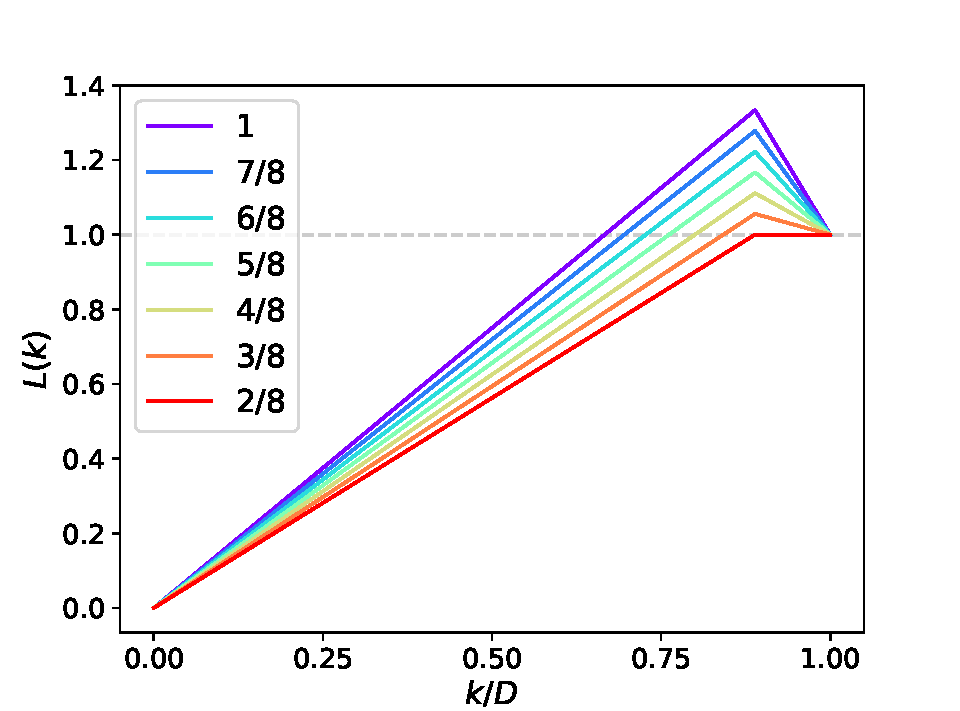
\includegraphics[height=3cm]{figs/negmasking_rho_strange_lc.pdf}
    %\caption{Maximally mixed state $\frac{1}{3}\id$}%
    }\hspace{8pt}%
    \subfigure[][]{%
    \label{fig:test2}%
    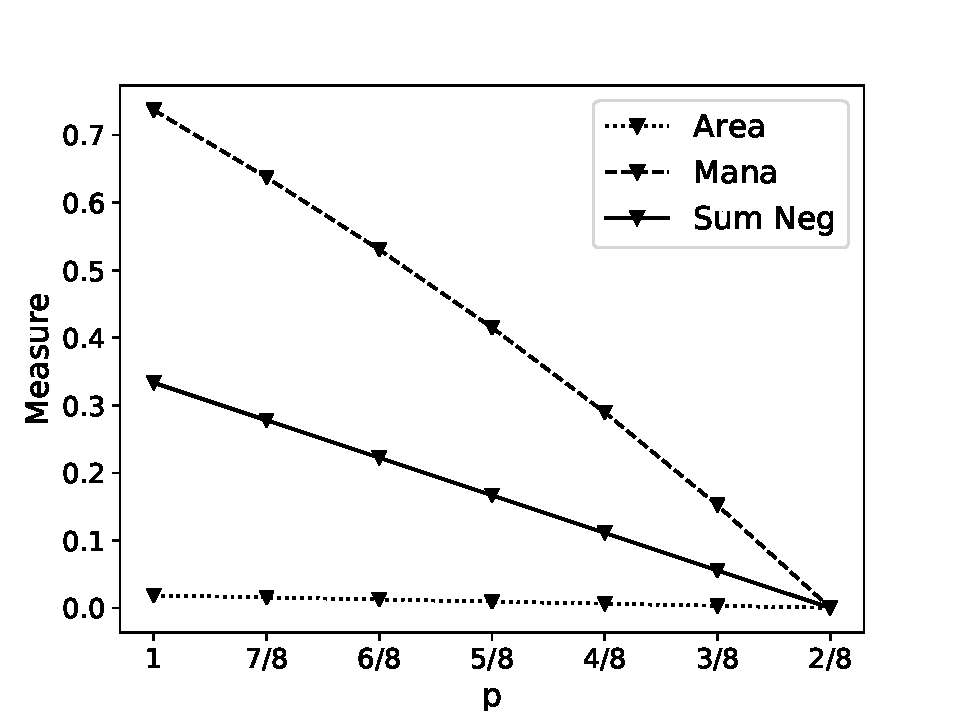
\includegraphics[height=3cm]{figs/negmasking_rho_strange_meas.pdf}
    %\caption{Zero state $\ketbra{0}{0}$}%
    }
    \caption{\subref{fig:test1} Lorenz curve of $p\ketbra{\rm{S}} + (1-p) \frac{1}{d}\id$ for $p$ given in the legend.\subref{fig:test2} Different measures for the states on the left. \\
    \nick{can replace~\cref{fig:lctoy} with a more informative version of this figure}
    }%
    \label{fig:test}
\end{figure}

Let $L_{>1}$ be the set of points on the Lorenz curve $\lc{\rho}{\sigma}(k)$ that lie above $1$ of state $\rho$ in the $\sigma$--fragment. 
If $\rho$ is a free state, $L_{>1}$ is empty and $\A_\sigma(\rho) = 0$. 
Otherwise, $\A_\sigma(\rho) > 0$ and it can be calculated exactly using the trapezium rule or the shoelace formula. 
Let $k$ be the index of the first point $\left(x_k, \lc{\rho}{\sigma}(k)\right)$ lying above $1$. 
Then $L_\rho(k)$ crosses $1$ at
\begin{equation}
	x_{\rm{int}} = x_k - \frac{x_k - x_{k-1}}{\lc{\rho}{\sigma}(k) - \lc{\rho}{\sigma}(k-1)}\lc{\rho}{\sigma}(k),\vspace{10pt}
\end{equation}
as well as at $\left(x_d, \lc{\rho}{\sigma}(d)\right) = (1,1)$

Now we can define
\begin{equation}
L_{>1}^+ = \{ (x_i, y_i) \}_{0 \leq i \leq n}
\end{equation}
such that it contains the initial point of intersection $(x_0, y_0) \equiv (x_{n+1}, y_{n+1}) \coloneqq (x_{\rm{int}}, 1)$, all points $(x_i, y_i)$, labelled by $i=1,\dots,n-1$ that lie above $y=1$ contained in $L_{>1}$ and finally the second point of intersection $(x_n, y_n) = (1,1)$.
Then, 
\begin{equation}
	\A_\sigma(\rho) = \frac{1}{2} \sum\limits_{i=0}^n (x_{i+1} y_i - x_i y_{i+1}).
\end{equation}

\section{Technical derivations for standard Lorenz curves}
\label{app:lcsu_technical}

\subsection{Binomial distributions and error bounds}\label{app:phi}
Consider an experiment consisting of $n$ trials of throwing a $p$-coin, that is a coin with probability $p$ of landing on one side and $1-p$ of landing on the other.
This scenario describes the construction of an $n$-copy Strange state Wigner distribution from a single-copy as presented in~\cref{sec:lcsu}.
The experiment is described by binomial statistics and we write down the sum over an even number of successful trials $\Phi_+$ (over an odd number of successful trials $\Phi_-$),
\begin{align}	
	\Phi_+(\mmf; \nnf, p) &\coloneqq \sum\limits_{\dummy=0}^{\mmf/2} \binom{\nnf}{2\dummy} p^{2\dummy} (1-p)^{\nnf-2\dummy}, \nonumber\\ 
	&\text{for even integers } \mmf\in[0,\nnf], \label{eq:fp_app} \\
	\Phi_-(\mmf; \nnf, p) &\coloneqq \sum\limits_{\dummy=1}^{(\mmf-1)/2} \binom{\nnf}{2\dummy+1} p^{2\dummy+1} (1-p)^{\nnf-(2\dummy+1)}, \nonumber\\ 
	&\text{for odd integers } \mmf\in[0,\nnf]. \label{eq:fn_app}
\end{align}
Note that index $\mmf$ only takes even (odd) values when labelling $\Phi_+$ ($\Phi_-$).
In~\cref{app:lcsu_coord_elb}, we will use $\Phi_+$ and $\Phi_-$ to express the elbow coordinates of standard Lorenz curves.

We define the classical entropy of a $p$-coin as well as the classical relative entropy between a $p$-coin and a $q$-coin,
\begin{align}
	S(p) &\coloneqq -p\log{p} -(1-p)\log{(1-p)}, \label{eq:ent}\\
	\ent{p}{q} &\coloneqq p \log{\frac{p}{q}} + (1-p) \log{\frac{1-p}{1-q}}. \label{eq:ent_rel}
\end{align}
They are symmetric in the sense that $S(p) = S(1-p)$ and $\ent{p}{q} = \ent{1-p}{1-q}$.

A useful result is the entropic bound on a combination~\cite{cit:ash}.
\begin{lemma}\label{lem:comb_bounds}
	For all $\dummy\in [1,\nnf-1]$,
	\begin{align}
		&\left[ 8\dummy\left(1-\frac{\dummy}{\nnf}\right) \right]^{-\frac{1}{2}} 2^{\nnf S\left(\frac{\dummy}{\nnf}\right)} \leq \binom{\nnf}{\dummy} \leq \\
		&\left[ 2\pi \dummy\left(1-\frac{\dummy}{\nnf}\right) \right]^{-\frac{1}{2}} 2^{\nnf S\left(\frac{\dummy}{\nnf}\right)}.
	\end{align}
\end{lemma}
\begin{proof}
	For $\dummy = 1,2, \nnf-1, \nnf-2$ check by direct calculation.	
	For all other cases, use Stirling's approximation. 
	\nick{CITE}
\end{proof}
With the help of this lemma, we directly arrive at 
\begin{theorem}\label{thm:bounds_strict}
	Given fixed $n>0$ and $p$, $\Phi_+, \Phi_-$ satisfy the following bounds:
	\begin{align*}
		\begin{split}
		&\text{1. } \Phi_+(\mmf; \nnf, p) \geq \sum\limits_{\dummy=0}^{\mmf/2}\left[ 16\dummy\left(1-\frac{2\dummy}{\nnf}\right) \right]^{-\frac{1}{2}} 2^{-\nnf\ent{\frac{2\dummy}{\nnf}}{p}}, \\
		&\hspace{14pt} \text{for all even } \mmf\in [2,\nnf] \\
		&\text{2. } \Phi_+(\mmf; \nnf, p) \leq \sum\limits_{\dummy=0}^{\mmf/2}\left[ 4\pi\dummy\left(1-\frac{2\dummy}{\nnf}\right) \right]^{-\frac{1}{2}} 2^{-\nnf\ent{\frac{2\dummy}{\nnf}}{p}}, \\
		&\hspace{14pt} \text{for all even } \mmf\in [2,\nnf] \\
		&\text{3. } \Phi_-(\mmf; \nnf, p) \geq \sum\limits_{\dummy=1}^{(\mmf-1)/2}\left[ 16(\dummy+1)\left(1-\frac{2\dummy+1}{\nnf}\right) \right]^{-\frac{1}{2}} \times \\
		&\hspace{14pt} \times 2^{-\nnf\ent{\frac{2\dummy+1}{\nnf}}{p}},\ \text{for all odd }\mmf\in [1,\nnf] \\
		&\text{4. } \Phi_-(\mmf; \nnf, p) \leq \sum\limits_{\dummy=1}^{(\mmf-1)/2}\left[ 4\pi(\dummy+1)\left(1-\frac{2\dummy+1}{\nnf}\right) \right]^{-\frac{1}{2}} \times \\
		&\hspace{14pt} \times 2^{-\nnf\ent{\frac{2\dummy+1}{\nnf}}{p}},\ \text{for all odd } \mmf\in [1,\nnf]
		\end{split}
	\end{align*}
\end{theorem}
\begin{proof}
	All four statements follow from application of~\cref{lem:comb_bounds} on the combinatorial coefficient and the defintion of relative entropy given in~\cref{eq:ent_rel}
\end{proof}

\iffalse % LOOSE BOUNDS & PLOT - START
The experiment is described by binomial statistics and we define the left tail of the cumulative binomial distribution,
\begin{equation}\label{eq:phil}
	\Phi_\ell(m; n, p) \coloneqq \sum\limits_{j=0}^m \binom{n}{j} p^j (1-p)^{n-j},
\end{equation}
where $m\in [0,n]$. 

The symmetry between the left tail of a $p$-coin distribution and the right tail of a $(1-p)$-coin distribution dictates that
\begin{align}\label{eq:phi_reverse}
	\Phi_\ell(m; n, p) + \Phi_\ell(n-m-1; n, 1-p) &= 1,\ m\in [0,n-1],
\end{align}
Entropic bounds on $\Phi_\ell$~\cite{cit:ash}.
\begin{lemma}\label{lem:phil_bounds}
	Given fixed $n>0$ and $p$, $\Phi_\ell$ satisfies the following bounds:
	\begin{align*}
		\begin{split}
		&\text{1. } \Phi_\ell(m; n, p) \geq \left[ 8m\left(1-\frac{m}{n}\right) \right]^{-\frac{1}{2}} 2^{-n\ents},\ m\in [1,n-1] \\
		&\text{2. } \Phi_\ell(m; n, p) \leq 2^{-n\ents},\ m\in [0,np] \\
		&\text{3. } \Phi_\ell(m; n, p) \leq 1 - \left[ 8(m+1)\left(1-\frac{m+1}{n}\right) \right]^{-\frac{1}{2}} 2^{-n\ent{\frac{m+1}{n}}{p}}, \\
		&\hspace{14pt} m\in [0,n-2]
		\end{split}
		\\
		&\text{4. } \Phi_\ell(m; n, p) \geq 1 - 2^{-n\ent{\frac{m+1}{n}}{p}},\ m\in [np+1,n-2]
	\end{align*}
\end{lemma}
\begin{proof}
	\nick{cite proof}
\end{proof}
Loose bounds follow
\begin{lemma}\label{lem:bounds_loose}
	Given fixed $n>0$ and $p$, $\Phi$ satisfies the following bounds:
	\begin{align*}
		\begin{split}
		&\text{1. } \Phi_{\pm}(m; n, p) \geq \left[ 8m\left(1-\frac{m}{n}\right) \right]^{-\frac{1}{2}} 2^{-n\ents},\ m\in [1,n-1] \\
		&\text{2. } \Phi_{\pm}(m; n, p) \leq 2^{-n\ents},\ m\in [0,np] \\
		&\text{3. } \Phi_{\pm}(m; n, p) \leq 1 - \left[ 8(m+1)\left(1-\frac{m+1}{n}\right) \right]^{-\frac{1}{2}} 2^{-n\ent{\frac{m+1}{n}}{p}}, \\
		&\hspace{14pt} m\in [0,n-2]
		\end{split}
	\end{align*}
\end{lemma}
\begin{proof}
	\nick{paste proof}
\end{proof}

We can therefore use~\cref{lem:bounds_loose,lem:bounds_strict} to bound the standard Lorenz curves.
\begin{figure}[b]
    \centering
    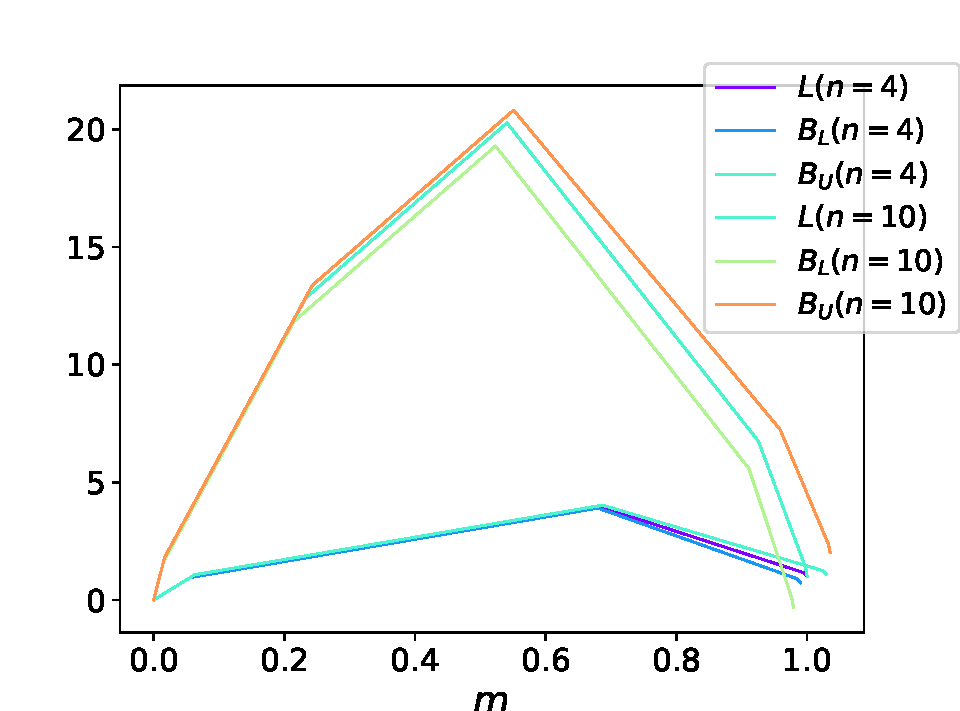
\includegraphics[scale=0.4]{figs/lc_bounds.pdf}
    \caption{\textbf{Lorenz curves and bounding curves.} 
    The figure explores the distillation process of a 10-copy $0.25$-noisy Strange state to a 4-copy $0.05$-noisy Strange state in the unital fragment.
    Clearly, by looking at the Lorenz curves, the distillation process is possible.
    However the bounding curves, derived in~\cref{lem:bounds_strict}, intersect at the end, suggesting that the process is not necessarily possible.
    }
    \label{fig:lc_bounds}
\end{figure}
\fi % LOOSE BOUNDS & PLOT - END

\subsection{Standard Lorenz curve elbow coordinates}\label{app:lcsu_coord_elb}
The Wigner distribution of the $\NN$-copy qutrit maximally mixed state $\left(\id/3\right)\too{\NN}$ is the uniform distribution 
\begin{equation}\label{eq:wu}
	\W{\left(\id/3\right)\too{\NN}} = \Bigg( \overbrace{\frac{1}{9^\NN}, \dots, \frac{1}{9^\NN}}^{9^\NN} \Bigg).
\end{equation}
The Wigner distribution of the 1-copy $\epsilon$-noisy Strange state $\noisys(\epsilon)$ in the unital fragment is a permutation of 
\begin{equation}\label{eq:wsu}
	\W{\noisys(\epsilon)} = \Bigg( \overbrace{\frac{1}{6} - \frac{1}{18}\epsilon, \dots, \frac{1}{6} - \frac{1}{18}\epsilon}^8, \overbrace{-\frac{1}{3} + \frac{4}{9}\epsilon}^1 \Bigg)
\end{equation}
The two distinct components are plotted~\cref{fig:noisys} as a function of noise. 
It is clear that in the unital fragment the Strange state contains Wigner negativities in the regime $0 \leq \epsilon \leq \tfrac{3}{4}$.
\begin{figure}[h]
    \centering
    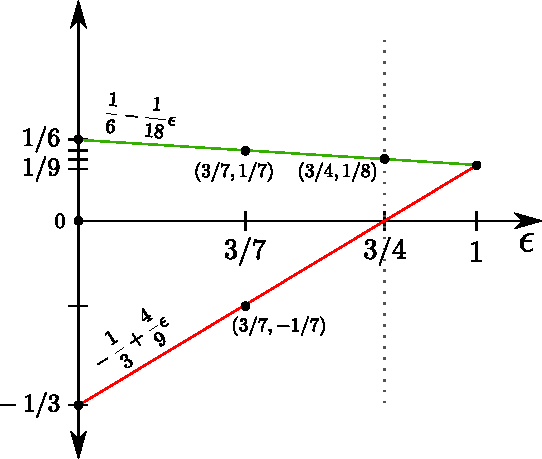
\includegraphics[scale=0.7]{figs/noisys.pdf}
    \caption{\textbf{Wigner components of the noisy Strange state.} 
    In the interval $0 \leq \epsilon < 3/7$, the negative component is larger than the positive components.
    At $\epsilon = 3/7$ the Wigner distribution is $(-\frac{1}{7},\frac{1}{7},\dots,\frac{1}{7})$.
    In the interval $3/7 < \epsilon < 3/4$, the positive components are larger than the negative component.
    In the interval $3/4 \leq \epsilon \leq 1$, there is no negativity.
    }
    \label{fig:noisys}
\end{figure}

The Wigner distribution of the $\NN$-copy $\epsilon$-noisy Strange state $\noisysN$ in the unital fragment is given by the convolution $\W{\noisysN} = \rm{W}_{\noisys(\epsilon)}\too{\NN}$.
In general, $\noisysN$ contains $\NN + 1$ distinct components, labelled $0,\dots, \NN$.
We present the distinct Wigner components of $\noisysN$ along with their multiplicites in~\cref{tab:lcsu}.
Note that LHS (RHS) refers to elbow coordinates $\ii$ on the left of and including (right of) the maximum, precisely
\begin{align}
&\text{LHS: } 0 \leq \ii \leq \frac{\lfloor \NN \rfloor}{2}; \\
&\text{RHS: } \frac{\lfloor \NN \rfloor}{2}+1 \leq \ii \leq \NN.
\end{align}
\begin{table}[h]
  \def\arraystretch{1.5}
  \centering
  \begin{tabular}{c|c|c|r|r}
    \multicolumn{3}{c|}{Case} & \multicolumn{1}{c}{$\mlt_{\ii}(\NN, \epsilon)$} & \multicolumn{1}{|c}{$w_{\ii}(\NN, \epsilon)$} \\[0.5ex]\hline
    \multirow{4}{*}{\raisebox{-4ex}{\rotatebox[origin=c]{90}{$0\leq \epsilon < \frac{3}{7}$}}} & \hspace{0.8ex}\multirow{2}{*}{\raisebox{-1ex}{\rotatebox[origin=c]{90}{$\NN$ even}}}\hspace{0.8ex} & LHS & $8^{2\ii}\binom{\NN}{2\ii}$ & $\left( \frac{1}{6} - \frac{1}{18}\epsilon \right)^{2\ii}\left( -\frac{1}{3} + \frac{4}{9}\epsilon \right)^{\NN-2\ii}$ \\
    & & RHS & $8^{\NN-2\ii}\binom{\NN}{2\ii}$ & $\left( \frac{1}{6} - \frac{1}{18}\epsilon \right)^{\NN-2\ii}\left( -\frac{1}{3} + \frac{4}{9}\epsilon \right)^{2\ii}$ \\ \cline{2-5}
    & \multirow{2}{*}{\raisebox{-2ex}{\rotatebox[origin=c]{90}{$\NN$ odd}}} & LHS & $8^{2\ii+1}\binom{\NN}{2\ii+1}$ & $\left( \frac{1}{6} - \frac{1}{18}\epsilon \right)^{2\ii+1}\left( -\frac{1}{3} + \frac{4}{9}\epsilon \right)^{\NN-2\ii-1}$ \\
    & & RHS & $8^{\NN-2\ii-1}\binom{\NN}{2\ii+1}$ & $\left( \frac{1}{6} - \frac{1}{18}\epsilon \right)^{\NN-2\ii-1}\left( -\frac{1}{3} + \frac{4}{9}\epsilon \right)^{2\ii+1}$ \\ \hline
    \multirow{4}{*}{\raisebox{-4ex}{\rotatebox[origin=c]{90}{$\frac{3}{7}\leq \epsilon < \frac{3}{4}$}}} & \multirow{2}{*}{\raisebox{-1ex}{\rotatebox[origin=c]{90}{$\NN$ even}}} & LHS & $8^{\NN-2\ii}\binom{\NN}{2\ii}$ & $\left( \frac{1}{6} - \frac{1}{18}\epsilon \right)^{\NN-2\ii}\left( -\frac{1}{3} + \frac{4}{9}\epsilon \right)^{2\ii}$ \\
    & & RHS & $8^{2\ii}\binom{\NN}{2\ii}$ & $\left( \frac{1}{6} - \frac{1}{18}\epsilon \right)^{2\ii}\left( -\frac{1}{3} + \frac{4}{9}\epsilon \right)^{\NN-2\ii}$ \\ \cline{2-5}
    & \multirow{2}{*}{\raisebox{-2ex}{\rotatebox[origin=c]{90}{$\NN$ odd}}} & LHS & $8^{\NN-2\ii}\binom{\NN}{2\ii}$ & $\left( \frac{1}{6} - \frac{1}{18}\epsilon \right)^{\NN-2\ii}\left( -\frac{1}{3} + \frac{4}{9}\epsilon \right)^{2\ii}$ \\
    & & RHS & $8^{2\ii}\binom{\NN}{2\ii}$ & $\left( \frac{1}{6} - \frac{1}{18}\epsilon \right)^{2\ii}\left( -\frac{1}{3} + \frac{4}{9}\epsilon \right)^{\NN-2\ii}$ \\ \hline
  \end{tabular}
  \caption{Wigner components $w_{\ii}(\NN, \epsilon)$ of $\noisysN$ along with their multiplicities $\mlt_{\ii}(\NN, \epsilon)$ in decreasing order in $\ii,\ 0 \leq \ii \leq \NN$.
  The order changes depending on the noise level $\epsilon$, the parity of the number of copies $\NN$ and the parity of the components (LHS vs RHS).
  Multiplication $2\ii$ is considered modulo $(\NN+1)$.}
  \label{tab:lcsu}
\end{table}

For example, the distribution of state $\noisys(0)\too{2}$ is
\begin{equation*}
	\begin{split}
	\rm{W}_{\noisys(0)\too{2}} = \Bigg( &\overbrace{\left( -\frac{1}{3} \right)^2}^1, \overbrace{\left( \frac{1}{6} \right)^2, \dots, \left( \frac{1}{6} \right)^2}^{64}, \\
	&\overbrace{ -\frac{1}{3} \cdot \frac{1}{6}, \dots, -\frac{1}{3} \cdot \frac{1}{6}}^{16} \Bigg)
	\end{split}
\end{equation*}

Every standard Lorenz curve contains $\NN$ elbows, labelled by 
\begin{equation*}
\{(x_{\ii}, L_{\ii})\}_{\ii=-1,0,\dots,\NN}\ ,
\end{equation*}
where the boundary points $(x_{-1}, L_{-1}) = (0,0)$ and $(x_{\NN}, L_{\NN}) = (1,1)$ are also included.
The maximum is the $(\lfloor \NN \rfloor/2)$-th elbow and its coordinates are calculated by collecting all the positive Wigner components,
\begin{align}
	x_{\lfloor \NN \rfloor/2} &= \frac{1}{2}\left(1 + \left(\frac{7}{9}\right)^\NN\right), \\
	L_{\lfloor \NN \rfloor/2} &= \frac{1}{2}\left (1 + \left(\frac{15 - 8\epsilon}{9}\right)^\NN \right).
\end{align}
%\sum_{j: even}^n a^j \binom{n}{j} = \frac{1}{2} [ (1+a)^n + (1-a)^n ]

Expressions for all the elbow coordinates follow from summing up the Wigner components in decreasing order and we present the elbow coordinates for standard Lorenz curves in~\cref{tab:lcsu_coord_elb_app}.
\begin{table}[h]
  \def\arraystretch{1.5}
  \centering
  \begin{tabular}{c|c|c|r|r}
    \multicolumn{3}{c|}{Case} & \multicolumn{1}{c}{$x_{\ii}$} & \multicolumn{1}{|c}{$L_{\ii}$} \\[0.5ex]\hline
    \multirow{4}{*}{\raisebox{-5ex}{\rotatebox[origin=c]{90}{$0\leq \epsilon < \frac{3}{7}$}}} & \hspace{0.8ex}\multirow{2}{*}{\raisebox{-3ex}{\rotatebox[origin=c]{90}{$\NN$ even}}}\hspace{0.8ex} & LHS & $\Phi_+\left(2\ii;\NN,\frac{8}{9}\right)$ & $\left( \frac{5}{3} - \frac{8}{9}\epsilon\ \right)^\NN \Phi_+\left(2\ii;\NN,\frac{12-4\epsilon}{15-8\epsilon}\right)$ \\
    & & RHS & $x_{\NN/2} + \Phi_-\left(2\ii;\NN,\frac{1}{9}\right)$ & $L_{\NN/2} - \left( \frac{5}{3} - \frac{8}{9}\epsilon\ \right)^\NN\Phi_-\left(2\ii;\NN,\frac{3-4\epsilon}{15-8\epsilon}\right)$ \\ \cline{2-5}
    & \multirow{2}{*}{\raisebox{-3ex}{\rotatebox[origin=c]{90}{$\NN$ odd}}} & LHS & $\Phi_-\left(2\ii;\NN,\frac{8}{9}\right)$ & $\left( \frac{5}{3} - \frac{8}{9}\epsilon\ \right)^\NN \Phi_-\left(2\ii;\NN,\frac{12-4\epsilon}{15-8\epsilon}\right)$ \\
    & & RHS & $x_{\NN/2} + \Phi_-\left(2\ii;\NN,\frac{1}{9}\right)$ & $L_{\NN/2} - \left( \frac{5}{3} - \frac{8}{9}\epsilon\ \right)^\NN\Phi_-\left(2\ii;\NN,\frac{3-4\epsilon}{15-8\epsilon}\right)$ \\ \hline
    \multirow{4}{*}{\raisebox{-5ex}{\rotatebox[origin=c]{90}{$\frac{3}{7}\leq \epsilon < \frac{3}{4}$}}} & \multirow{2}{*}{\raisebox{-3ex}{\rotatebox[origin=c]{90}{$\NN$ even}}} & LHS & $\Phi_+\left(2\ii;\NN,\frac{1}{9}\right)$ & $\left( \frac{5}{3} - \frac{8}{9}\epsilon\ \right)^\NN \Phi_+\left(2\ii;\NN,\frac{3-4\epsilon}{15-8\epsilon}\right)$ \\
    & & RHS & $x_{\NN/2} + \Phi_-\left(2\ii;\NN,\frac{8}{9}\right)$ & $L_{\NN/2} - \left( \frac{5}{3} - \frac{8}{9}\epsilon\ \right)^\NN\Phi_-\left(2\ii;\NN,\frac{12-4\epsilon}{15-8\epsilon}\right)$ \\ \cline{2-5}
    & \multirow{2}{*}{\raisebox{-3ex}{\rotatebox[origin=c]{90}{$\NN$ odd}}} & LHS & $\Phi_+\left(2\ii;\NN,\frac{1}{9}\right)$ & $\left( \frac{5}{3} - \frac{8}{9}\epsilon\ \right)^\NN \Phi_+\left(2\ii;\NN,\frac{3-4\epsilon}{15-8\epsilon}\right)$ \\
    & & RHS & $x_{\NN/2} + \Phi_+\left(2\ii;\NN,\frac{8}{9}\right)$ & $L_{\NN/2} - \left( \frac{5}{3} - \frac{8}{9}\epsilon\ \right)^\NN\Phi_+\left(2\ii;\NN,\frac{12-4\epsilon}{15-8\epsilon}\right)$ \\ \hline
  \end{tabular}
  \caption{Standard Lorenz curves elbow coordinates.
  The expresion depends on the noise level $\epsilon$, the parity of the number of copies $\NN$ and the location of the elbow relative to the maximum (LHS vs RHS).
  Multiplication $2\ii$ is considered modulo $(\NN+1)$.
  Note that the Lorenz curve boundary points are $(x_{-1}, L_{-1}) \coloneqq (0,0)$ and $(x_{\NN}, L_{\NN}) = (1,1)$.
  }
  \label{tab:lcsu_coord_elb_app}
\end{table}

\subsection{Standard Lorenz curve coordinates}\label{app:lcsu_coord}
We can get explicit expressions for all $9^{\NN}$ points of the standard Lorenz curve $\lc{\noisysN}{\id/3}$, in terms of the elbow coordinates:
\begin{align}
    x_{\ii\jj} &= \left( 1-\frac{\jj}{\mlt_{\ii}} \right) x_{\ii-1} + \frac{\jj}{\mlt_{\ii}} x_{\ii}, \label{eq:x}\\
    L_{\ii\jj} &= \left( 1-\frac{\jj}{\mlt_{\ii}} \right) L_{\ii-1} + \frac{\jj}{\mlt_{\ii}} L_{\ii} \label{eq:l}
\end{align}
for $\jj = 1,\dots,\mlt_{\ii}$ and $\ii=0,\dots,\NN$, where multiplicities $\mlt_\ii = \mlt_\ii(\NN, \epsilon)$ are given in~\cref{tab:lcsu}.

For visualisation purposes, we plot the Lorenz curve of state $\noisys(0)\too{2}$.
\begin{figure}[t]
    \centering
    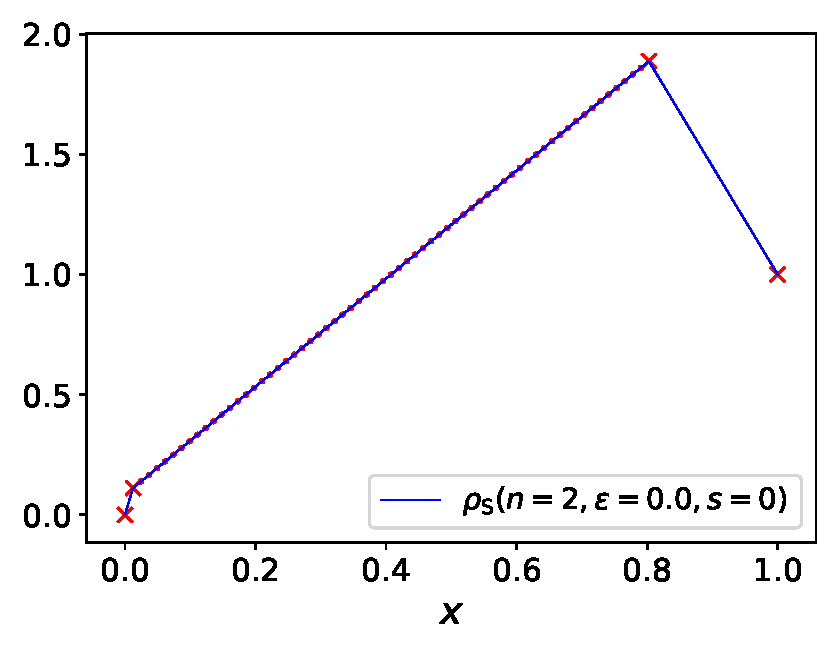
\includegraphics[scale=0.6]{figs/lcpoints.pdf}
    \caption{\textbf{All points on the Lorenz curve are uniformly distributed.}
    \cref{eq:x,eq:l}) capture the coordinates of all points up to the maximum.
    }
    \label{fig:lc}
\end{figure}

Consider the state 
\begin{equation*}
    \noisys(\epsilon)\too{\tt} \otimes \left( \frac{1}{3}\id \right)\too{\mm},
\end{equation*} %\noisys(\tt, \epsilon, \mm) \coloneqq 
with $\tt + \mm = \NN$.

Tensoring with the maximally mixed state keeps the Lorenz curve unchanged, but increases the resolution of (the uniformly distributed) points.
The new point coordinates are given by:
\begin{align}
    &x_{\ii\jj\kk} = \left( 1-p_{\ii\jj\kk}\right) x_{\ii-1} + p_{\ii\jj\kk} x_{\ii} \label{eq:lcsu_xcoord}\\
    &L_{\ii\jj\kk} = \left( 1-p_{\ii\jj\kk} \right) L_{\ii-1} + p_{\ii\jj\kk} L_{\ii}, \label{eq:lcsu_lcoord}\\
    &\text{where } p_{\ii\jj\kk} = \frac{\kk + (\jj-1)9^{\mm}}{9^{\mm} \mlt_{\ii}} \nonumber\\
    &\text{for } \ii=0,\dots,\tt,\ \jj = 1,\dots,\mlt_{\ii}(\tt, \epsilon') \text{ and } \kk = 1,\dots,9^{\mm}. \nonumber
\end{align}

We can unify the indices, by introducing a single index
\begin{equation}
    \II(\ii,\jj,\kk) \coloneqq \kk + \left[ (\jj-1) + \sum_{\dummy=0}^{\ii-1} \mlt_{\dummy}(\tt, \epsilon') \right]9^{\mm},
\end{equation}
so that $\II=1,2,\dots, 9^{\NN}$.
The elbow coordinates correspond to 
\begin{equation}
	\II(\ii, \mlt_{\ii}(\tt, \epsilon'), 9^{\mm}) = \sum_{\dummy=0}^{\ii} \mlt_{\dummy}(\tt, \epsilon'),\ \ii= 0,\dots,\tt.
\end{equation}
The index function $\II$ is bijective, i.e.
\begin{equation}
	(\ii,\jj,\kk) = (\ii',\jj',\kk') \Leftrightarrow \II(\ii,\jj,\kk) = \II(\ii',\jj',\kk').
\end{equation}

\subsection{Strange state MSD in the unital fragment}\label{app:lc_compare}
Consider the Strange state MSD process in the unital fragment,
\begin{equation}\label{eq:su_conversion}
    \noisysn \xrightarrow{\mathcal{O}_{\id/3}} \noisys(\tt, \epsilon', \mm),\ \nn = \tt + \mm.
\end{equation}
We denote initial state indices without a prime and target state indices with a prime,
\begin{align}
    \II(\ii,\jj,\kk=1) &= \jj + \sum_{\dummy=0}^{\ii-1} \mlt_{\dummy}(\nn, \epsilon), \\
    \II'(\ii',\jj',\kk') &= \kk' + \left[ (\jj'-1) + \sum_{\dummy=0}^{\ii'-1} \mlt_{\dummy}(\tt, \epsilon') \right]9^{\mm}.
\end{align}

Pointwise Lorenz curve comparison requires $x_{\II} = x_{\II'}$, so the question is: 
\begin{center}
\emph{Given a triplet $(\ii',\jj',\kk')$, what is the tuple $(\ii,\jj)$ such that $\II(\ii,\jj) = \II'(\ii',\jj',\kk')$?}
\end{center}

According to~\cref{thm:elbows} which is proved in~\cref{app:lc_constraints}, for standard Lorenz curves, we need to match indices at the target state elbows, so the requirement on the indices is finding a tuple $(\ii, \jj)$, such that for a given $\ii' = 0,\dots,\tt$,
\begin{equation}
	\jj + \sum_{\dummy=0}^{\ii-1} \mlt_{\dummy}(\nn, \epsilon) = \sum_{\dummy=0}^{\ii'} \mlt_{\dummy}(\tt, \epsilon').
\end{equation}

As a basic example, consider the process 
\begin{equation}
\rho_{\rm{S}}(\epsilon)\too{4} \xrightarrow{\mathcal{O}_{\id/3}} \rho_{\rm{S}}(\epsilon')\too{2} \otimes \left( \frac{1}{3}\id \right)\too{2}.
\end{equation}
We want to check which Lorenz curve is higher at the first elbows of the target state, i.e. we want to verify or reject the first inequality below:
\begin{equation}
	L_{\II(\ii,\jj)} \geq L'_{\II'(0, 1, 81)}
\end{equation}
where the first multiplicity of the target state is $m_0 = 1$.
The multiplicities of the initial state are $(1, 384, 4096)$.

The challenge is to find $\ii,\jj$ such that $i(\ii,\jj) = i'(0,1,81)$.
\nick{By trial and error}, we find that $(\ii,\jj) = (1, 80)$.
Now we can use~\cref{eq:lcsu_lcoord} to directly calculate
\begin{align*}
	L'_{i'(0,1,81)} &= L'_0 = \left( \frac{5}{3} - \frac{8}{9}\epsilon\ \right)^2 \Phi_+\left(0;2,4\frac{3-\epsilon}{15-8\epsilon}\right), \\
	L_{i(1, 80)} &= \left(1-\frac{80}{384} \right) L_0 + \frac{80}{384} L_1 \\
	\begin{split}
	&= \left( \frac{5}{3} - \frac{8}{9}\epsilon\ \right)^4 \bigg[ \frac{19}{24} \Phi_+\left(0;4,4\frac{3-\epsilon}{15-8\epsilon}\right) \\ 
	&\qquad + \frac{5}{24}\Phi_+\left(2;4,4\frac{3-\epsilon}{15-8\epsilon}\right) \bigg],
	\end{split}
\end{align*}
and then compare them.

\subsection{Lorenz curve independent constraints}\label{app:lc_constraints}

\begin{theorem}
	Let $\rho, \tau$ be two quantum states with Lorenz curves $\lc{\rho}{\sigma}(x), \lc{\tau}{\sigma}(x)$ in the $\sigma$-fragment.
	
	Let $\tt$ be the number of elbows of $\lc{\tau}{\sigma}(x)$ and $E \coloneqq \{x_1, \dots, x_\tt\}$ be their locations.
	
	Then, $\lc{\rho}{\sigma}(x) \geq \lc{\tau}{\sigma}(x)$ for all $x \in [0,1]$ iff $\lc{\rho}{\sigma}(x_{\ii}) \geq \lc{\tau}{\sigma}(x_{\ii})$ for all $\ii =1,\dots,\tt$.
\end{theorem}
\begin{proof}	
	$\lc{\rho}{\sigma}(x) \geq \lc{\tau}{\sigma}(x)$ for all $x \in [0,1]$ trivially implies $\lc{\rho}{\sigma}(x_{\ii}) \geq \lc{\tau}{\sigma}(x_{\ii})$ for all $\ii = 1,\dots,\tt$.
	
	Conversely, assume that $\lc{\rho}{\sigma}(x_{\ii}) \geq \lc{\tau}{\sigma}(x_{\ii})$ for all $\ii = 1,\dots,r$.
	First, let $x_0 = 0$ and $x_{\tt+1} = 1$, so that $\lc{\rho}{\sigma}(x_0) = \lc{\tau}{\sigma}(x_0) = 0$ and $\lc{\rho}{\sigma}(x_{\tt+1}) = \lc{\tau}{\sigma}(x_{\tt+1}) = 1$.
	Hence, we can extend the set of elbows $E$ to $E' = E \cup \{x_0, x_{\tt+1}\}$.
	
	Pick two consecutive locations $x_{\ii}, x_{\ii+1}$ in $E'$ and consider the line segment $\ell_\tau(x)$ connecting points $(x_{\ii}, \lc{\tau}{\sigma}(x_{\ii}))$ and $(x_{\ii+1}, \lc{\tau}{\sigma}(x_{\ii+1}))$ as well as the line segment $\ell_\rho(x)$ connecting points $(x_{\ii}, \lc{\rho}{\sigma}(x_{\ii}))$ and $(x_{\ii+1}, \lc{\rho}{\sigma}(x_{\ii+1}))$.
	This is illustrated in~\cref{fig:elbows_proof}.
\begin{figure}[h]
    \centering
    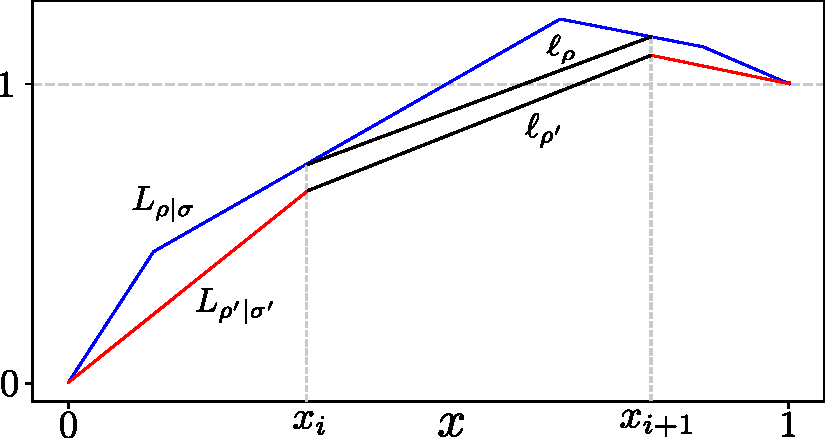
\includegraphics[scale=0.6]{figs/elbows_proof.pdf}
    \caption{\textbf{Illustration of~\cref{thm:elbows}}.
    }
    \label{fig:elbows_proof}
\end{figure}

	Due to concavity of $\lc{\rho}{\sigma}$, it is clear that for all $x \in [x_{\ii}, x_{\ii+1}]$, we have $\lc{\rho}{\sigma}(x) \geq \ell_\rho(x) \geq \ell_\tau(x) = \lc{\tau}{\sigma}(x)$.
	This argument can be made in all intervals $[x_{\ii}, x_{\ii+1}]$ with $\ii=0,\dots,\tt$, so the proof is complete.
\end{proof}
This theorem is of practical importance in calculating the necessary distillation constraints derived via majorization.

In particular, it can be used in the discussion of standard Lorenz curves to set the necessary constraints,
\begin{align}
L\left(x_{\II'(0, \mlt'_{0}, 9^{\mm})}\right) &\geq L\left(x_{\II'(0, m'_{0}, 9^{\mm})}\right), \nonumber\\
L\left(x_{\II'(1, \mlt'_{1}, 9^{\mm})}\right) &\geq L\left(x_{\II'(1, m'_{1}, 9^{\mm})}\right), \nonumber\\
&\vdotswithin{=} \nonumber\\
L\left(x_{\II'(\tt, \mlt'_{r}, 9^{\mm})}\right) &\geq L\left(x_{\II'(\tt, m'_{\tt}, 9^{\mm})}\right), \nonumber
\end{align}
where $x_{\II'(0, \mlt'_{0}, 9^{\mm'})}, x_{\II'(1, \mlt'_{1}, 9^{\mm'})}, \dots, x_{\II'(\tt, \mlt'_{\tt}, 9^{\mm'})} \in T$ are the locations of the elbows of $\lc{\rho_{\rm{S}}(\epsilon')\too{\tt}}{\frac{1}{d}\id}$ (excluding $0$ and $1$).



